documentclass{article}
\usepackage{tikz}
\usetikzlibrary{calc, arrows.meta, decorations.markings, patterns, shapes.geometric, positioning, 3d}
\usepackage{amsmath, amssymb}

\begin{document}

% ============================================================================
% FIGURE 1: Principal Bundle Architecture
% ============================================================================
\begin{figure}[h]
\centering
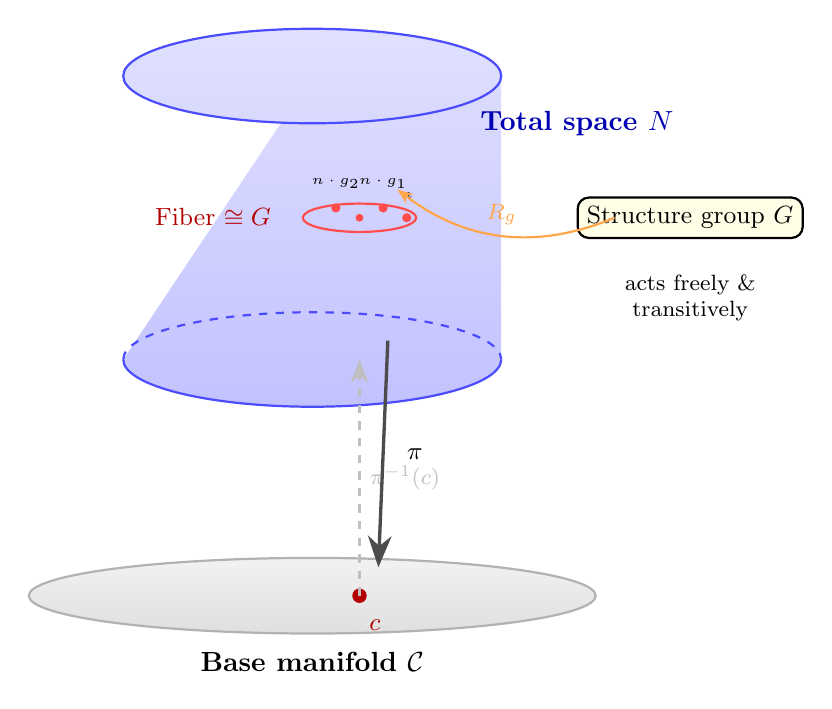
\begin{tikzpicture}[scale=1.2, every node/.style={font=\small}]

% Total space N (cylinder representing bundle)
\shade[top color=blue!20, bottom color=blue!40, opacity=0.6]
  (0,3) ellipse (2 and 0.5)
  -- (-2,0) arc (180:360:2 and 0.5)
  -- (2,3) arc (0:180:2 and 0.5);
\draw[thick, blue!70] (0,3) ellipse (2 and 0.5);
\draw[thick, blue!70] (-2,0) arc (180:360:2 and 0.5);
\draw[thick, blue!70, dashed] (-2,0) arc (180:0:2 and 0.5);

% Label total space
\node[blue!70!black, font=\bfseries] at (2.8,2.5) {Total space $N$};

% Base manifold C
\shade[top color=gray!10, bottom color=gray!25]
  (0,-2.5) ellipse (3 and 0.4);
\draw[thick, gray!60] (0,-2.5) ellipse (3 and 0.4);
\node[below, font=\bfseries] at (0,-3) {Base manifold $\mathcal{C}$};

% Pick a point c on base
\filldraw[red!70!black] (0.5,-2.5) circle (2pt);
\node[below right, red!70!black] at (0.5,-2.65) {$c$};

% Fiber above c
\coordinate (base) at (0.5,-2.5);
\coordinate (fiber_bottom) at (0.5,0);
\coordinate (fiber_top) at (0.5,3);

\draw[-{Stealth[length=3mm]}, thick, gray!50, dashed] 
  (base) -- (fiber_bottom) node[midway, right, font=\footnotesize] {$\pi^{-1}(c)$};

% Draw fiber as small circle
\draw[thick, red!70] (0.5,1.5) ellipse (0.6 and 0.15);
\filldraw[red!70] (0.5,1.5) circle (1pt);

% G-action on fiber
\node[red!70!black, left=8pt] at (-0.1,1.5) {Fiber $\cong G$};

% Show some points on fiber and G action
\foreach \angle/\label in {0/n, 60/n \cdot g_1, 120/n \cdot g_2} {
  \filldraw[red!70] ($(0.5,1.5) + (\angle:0.5 and 0.12)$) circle (1.2pt);
  \node[font=\tiny, above] at ($(0.5,1.5) + (\angle:0.5 and 0.12) + (0,0.1)$) {$\label$};
}

% Projection arrow
\draw[-{Stealth[length=4mm, width=3mm]}, very thick, black!70]
  (0.8,0.2) -- (0.7,-2.2);
\node[right, font=\small\bfseries] at (0.9,-1) {$\pi$};

% Structure group G (in a box)
\node[draw, thick, rounded corners, fill=yellow!10, font=\small] 
  at (4,1.5) {Structure group $G$};
\node[below, font=\footnotesize, text width=2.5cm, align=center] 
  at (4,1) {acts freely \& transitively};

% Show G action with curved arrow
\draw[-{Stealth[length=2mm]}, thick, orange!70, bend left=30]
  (3.2,1.5) to node[above, font=\footnotesize] {$R_g$} (0.9,1.8);

\end{tikzpicture}
\caption{%
\textbf{Principal Bundle Structure.} The total space $N$ is a $G$-bundle over base manifold $\mathcal{C}$ with projection $\pi: N \to \mathcal{C}$. Each fiber $\pi^{-1}(c) \cong G$ is a copy of the structure group, shown here at point $c \in \mathcal{C}$. The group $G$ acts freely and transitively on fibers via right multiplication $R_g$.
}
\label{fig:principal_bundle}
\end{figure}

% ============================================================================
% FIGURE 2: Associated Bundle Construction
% ============================================================================
\begin{figure}[h]
\centering
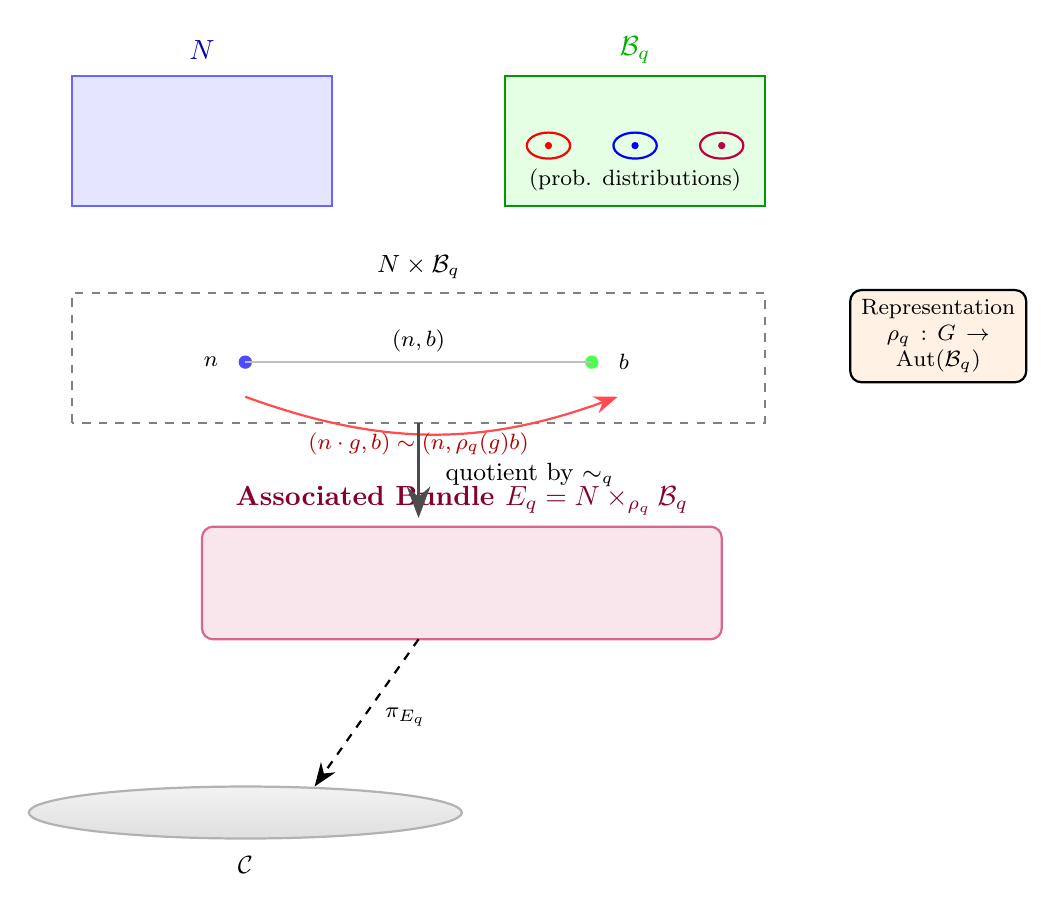
\begin{tikzpicture}[scale=1.1, every node/.style={font=\small}]

% Principal bundle N (simplified)
\draw[thick, blue!60, fill=blue!10] 
  (-1,4) rectangle (2,5.5);
\node[blue!70!black, font=\bfseries] at (0.5,5.8) {$N$};

% Typical fiber (statistical manifold)
\draw[thick, green!60!black, fill=green!10] 
  (4,4) rectangle (7,5.5);
\node[green!70!black, font=\bfseries] at (5.5,5.8) {$\mathcal{B}_q$};

% Draw some probability distributions in Bq
\foreach \x/\col in {4.5/red, 5.5/blue, 6.5/purple} {
  \draw[\col, thick] (\x,4.7) ellipse (0.25 and 0.15);
  \filldraw[\col] (\x,4.7) circle (1pt);
}
\node[font=\footnotesize] at (5.5,4.3) {(prob. distributions)};

% Product space N × Bq
\draw[thick, dashed, gray] 
  (-1,1.5) rectangle (7,3);
\node[font=\small\bfseries] at (3,3.3) {$N \times \mathcal{B}_q$};

% Show example element
\filldraw[blue!70] (1,2.2) circle (2pt);
\node[left, font=\footnotesize] at (0.8,2.2) {$n$};
\filldraw[green!70] (5,2.2) circle (2pt);
\node[right, font=\footnotesize] at (5.2,2.2) {$b$};
\draw[thick, gray!50] (1,2.2) -- (5,2.2);
\node[above, font=\footnotesize] at (3,2.2) {$(n,b)$};

% Equivalence relation
\draw[-{Stealth[length=3mm]}, thick, red!70, bend right=20] 
  (1,1.8) to (5.3,1.8);
\node[below, font=\footnotesize, red!70!black] at (3,1.5) 
  {$(n \cdot g, b) \sim (n, \rho_q(g)b)$};

% Associated bundle Eq
\draw[thick, purple!60, fill=purple!10, rounded corners] 
  (0.5,-1) rectangle (6.5,0.3);
\node[purple!70!black, font=\bfseries] at (3.5,0.6) 
  {Associated Bundle $E_q = N \times_{\rho_q} \mathcal{B}_q$};

% Quotient arrow
\draw[-{Stealth[length=4mm, width=3mm]}, very thick, black!70]
  (3,1.5) -- (3,0.4);
\node[right, font=\small] at (3.2,0.9) {quotient by $\sim_q$};

% Base manifold at bottom
\shade[top color=gray!10, bottom color=gray!25]
  (1,-3) ellipse (2.5 and 0.3);
\draw[thick, gray!60] (1,-3) ellipse (2.5 and 0.3);
\node[below, font=\small\bfseries] at (1,-3.4) {$\mathcal{C}$};

% Projection from Eq to C
\draw[-{Stealth[length=3mm]}, thick, dashed]
  (3,-1) -- (1.8,-2.7);
\node[right, font=\footnotesize] at (2.5,-1.9) {$\pi_{E_q}$};

% Representation box
\node[draw, thick, rounded corners, fill=orange!10, font=\footnotesize, text width=2cm, align=center] 
  at (9,2.5) {Representation\\$\rho_q: G \to \mathrm{Aut}(\mathcal{B}_q)$};

\end{tikzpicture}
\caption{%
\textbf{Associated Bundle Construction.} Starting from principal bundle $N$ and fiber $\mathcal{B}_q$ (statistical manifold), we form the product $N \times \mathcal{B}_q$ and quotient by the equivalence relation $(n \cdot g, b) \sim (n, \rho_q(g)b)$ induced by representation $\rho_q$. The resulting associated bundle $E_q$ projects to base $\mathcal{C}$.
}
\label{fig:associated_bundle}
\end{figure}

% ============================================================================
% FIGURE 3: SO(3) Action on Gaussian Manifold
% ============================================================================
\begin{figure}[h]
\centering
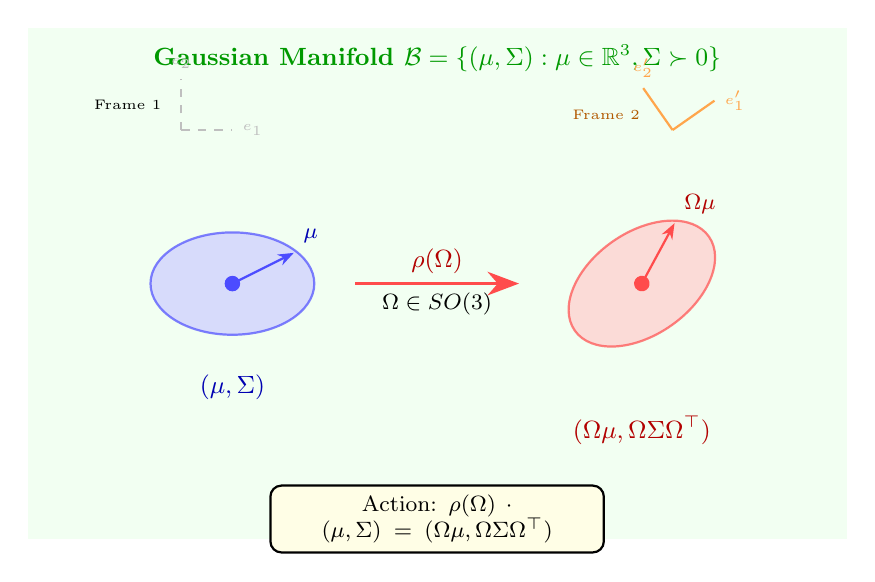
\begin{tikzpicture}[scale=1.3, every node/.style={font=\small}]

% Gaussian manifold background
\fill[green!5] (-1,-1) rectangle (7,4);
\node[green!60!black, font=\small\bfseries] at (3,3.7) 
  {Gaussian Manifold $\mathcal{B} = \{(\mu, \Sigma) : \mu \in \mathbb{R}^3, \Sigma \succ 0\}$};

% Original Gaussian (μ, Σ)
\begin{scope}[shift={(1,1.5)}]
  % Draw ellipsoid representing covariance
  \draw[thick, blue!70, fill=blue!20, opacity=0.7] 
    (0,0) ellipse (0.8 and 0.5);
  % Mean vector
  \filldraw[blue!70] (0,0) circle (2pt);
  \draw[-{Stealth[length=2mm]}, thick, blue!70] (0,0) -- (0.6,0.3);
  \node[above right, blue!70!black, font=\footnotesize] at (0.6,0.3) {$\mu$};
  % Label
  \node[below, blue!70!black, font=\small\bfseries] at (0,-0.8) {$(\mu, \Sigma)$};
\end{scope}

% SO(3) transformation arrow
\draw[-{Stealth[length=4mm, width=3mm]}, very thick, red!70]
  (2.2,1.5) -- (3.8,1.5);
\node[above, font=\small\bfseries, red!70!black] at (3,1.5) 
  {$\rho(\Omega)$};
\node[below, font=\footnotesize] at (3,1.5) {$\Omega \in SO(3)$};

% Transformed Gaussian (Ωμ, ΩΣΩᵀ)
\begin{scope}[shift={(5,1.5)}, rotate=35]
  % Draw rotated ellipsoid
  \draw[thick, red!70, fill=red!20, opacity=0.7] 
    (0,0) ellipse (0.8 and 0.5);
  % Transformed mean vector
  \filldraw[red!70] (0,0) circle (2pt);
  \draw[-{Stealth[length=2mm]}, thick, red!70] (0,0) -- (0.6,0.3);
  \node[above right, red!70!black, font=\footnotesize] at (0.6,0.3) {$\Omega\mu$};
\end{scope}
\node[below, red!70!black, font=\small\bfseries] at (5,0.3) 
  {$(\Omega\mu, \Omega\Sigma\Omega^{\top})$};

% Show the transformation formula in a box
\node[draw, thick, rounded corners, fill=yellow!10, font=\footnotesize, text width=4cm, align=center] 
  at (3,-0.8) {
    Action: $\rho(\Omega) \cdot (\mu, \Sigma) = (\Omega\mu, \Omega\Sigma\Omega^{\top})$
  };

% Show multiple gauge frames
\begin{scope}[shift={(0.5,3)}]
  \draw[thick, gray!50, dashed] (0,0) -- (0.5,0) node[right, font=\tiny] {$e_1$};
  \draw[thick, gray!50, dashed] (0,0) -- (0,0.5) node[above, font=\tiny] {$e_2$};
  \node[left, font=\tiny] at (-0.1,0.25) {Frame 1};
\end{scope}

\begin{scope}[shift={(5.3,3)}, rotate=35]
  \draw[thick, orange!70] (0,0) -- (0.5,0) node[right, font=\tiny] {$e_1'$};
  \draw[thick, orange!70] (0,0) -- (0,0.5) node[above, font=\tiny] {$e_2'$};
  \node[left, font=\tiny, orange!70!black] at (-0.1,0.25) {Frame 2};
\end{scope}

\end{tikzpicture}
\caption{%
\textbf{SO(3) Action on Gaussian Manifold.} The gauge group $G = SO(3)$ acts on the statistical manifold $\mathcal{B}$ of 3D Gaussian distributions via the representation $\rho(\Omega) \cdot (\mu, \Sigma) = (\Omega\mu, \Omega\Sigma\Omega^{\top})$. This rotates both the mean vector and covariance ellipsoid, corresponding to a change of reference frame. Different agents observe the same informational content in rotated local frames.
}
\label{fig:so3_action}
\end{figure}

% ============================================================================
% FIGURE 4: Multi-Agent Overlap and Communication
% ============================================================================
\begin{figure}[h]
\centering
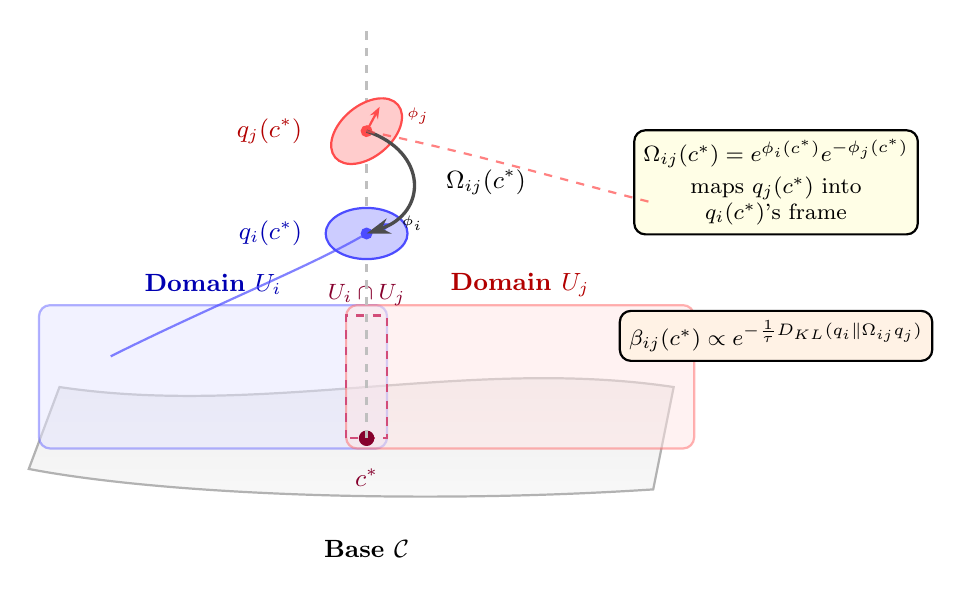
\begin{tikzpicture}[scale=1.3, every node/.style={font=\small}]

% Base manifold
\shade[top color=gray!15, bottom color=gray!5, draw=gray!60, thick]
  (0,0) .. controls (2,-0.3) and (4,0.3) .. (6,0)
  -- (5.8,-1.0) .. controls (3.5,-1.15) and (1.0,-1.05) .. (-0.3,-0.8)
  -- cycle;
\node[below, font=\small\bfseries] at (3,-1.4) {Base $\mathcal{C}$};

% Agent i domain
\draw[thick, blue!60, fill=blue!10, opacity=0.5, rounded corners]
  (-0.2,-0.6) rectangle (3.2,0.8);
\node[blue!70!black, font=\small\bfseries] at (1.5,1) {Domain $U_i$};

% Agent j domain  
\draw[thick, red!60, fill=red!10, opacity=0.5, rounded corners]
  (2.8,-0.6) rectangle (6.2,0.8);
\node[red!70!black, font=\small\bfseries] at (4.5,1) {Domain $U_j$};

% Overlap region
\draw[thick, purple!70, dashed] (2.8,-0.5) rectangle (3.2,0.7);
\node[purple!70!black, font=\footnotesize] at (3,0.9) {$U_i \cap U_j$};

% Point c* in overlap
\filldraw[purple!70!black] (3,-0.5) circle (2pt);
\node[below, purple!70!black, font=\small] at (3,-0.7) {$c^*$};

% Fibers at c*
\draw[thick, dashed, gray!50] (3,-0.5) -- (3,3.5);

% Agent i's section value
\begin{scope}[shift={(3,1.5)}]
  \draw[thick, blue!70, fill=blue!20] (0,0) ellipse (0.4 and 0.25);
  \filldraw[blue!70] (0,0) circle (1.5pt);
  \node[left=5pt, blue!70!black] at (-0.4,0) {$q_i(c^*)$};
  % Local frame
  \draw[-{Stealth[length=1.5mm]}, blue!70, thick] (0,0) -- (0.25,0.1);
  \node[right, font=\tiny] at (0.25,0.1) {$\phi_i$};
\end{scope}

% Agent j's section value
\begin{scope}[shift={(3,2.5)}, rotate=40]
  \draw[thick, red!70, fill=red!20] (0,0) ellipse (0.4 and 0.25);
  \filldraw[red!70] (0,0) circle (1.5pt);
  % Local frame
  \draw[-{Stealth[length=1.5mm]}, red!70, thick] (0,0) -- (0.25,0.1);
\end{scope}
\node[left=5pt, red!70!black] at (2.6,2.5) {$q_j(c^*)$};
\node[right, font=\tiny, red!70!black] at (3.3,2.65) {$\phi_j$};

% Transport operator Ωij
\draw[-{Stealth[length=3mm, width=2mm]}, very thick, black!70, line width=1.2pt]
  (3,2.5) .. controls (3.6,2.3) and (3.6,1.7) .. (3,1.5);
\node[right=3pt, font=\small\bfseries] at (3.6,2) {$\Omega_{ij}(c^*)$};

% Show the transformation formula
\node[draw, thick, rounded corners, fill=yellow!10, font=\footnotesize, align=center] 
  at (7,2) {
    $\Omega_{ij}(c^*) = e^{\phi_i(c^*)} e^{-\phi_j(c^*)}$\\[2pt]
    maps $q_j(c^*)$ into\\
    $q_i(c^*)$'s frame
  };

% Alignment weight β
\node[draw, thick, rounded corners, fill=orange!10, font=\footnotesize] 
  at (7,0.5) {
    $\beta_{ij}(c^*) \propto e^{-\frac{1}{\tau}D_{KL}(q_i \| \Omega_{ij}q_j)}$
  };

% Section curves
\draw[thick, blue!70, opacity=0.7] 
  (0.5,0.3) .. controls (1.5,0.8) and (2.5,1.2) .. (3,1.5);
\draw[thick, red!70, opacity=0.7, dashed] 
  (3,2.5) .. controls (4,2.3) and (5,2.0) .. (5.8,1.8);

\end{tikzpicture}
\caption{%
\textbf{Multi-Agent Communication via Gauge Transport.} Agents $i$ and $j$ have overlapping domains $U_i$ and $U_j$ on base manifold $\mathcal{C}$. At point $c^* \in U_i \cap U_j$, each agent has a belief $q_i(c^*), q_j(c^*)$ represented in their local gauge frames $\phi_i, \phi_j$. The transport operator $\Omega_{ij}(c^*) = e^{\phi_i}e^{-\phi_j}$ rotates agent $j$'s belief into agent $i$'s frame, enabling gauge-covariant alignment via KL divergence. The attention weight $\beta_{ij}$ quantifies alignment strength.
}
\label{fig:multi_agent_overlap}
\end{figure}










\end{document}